%%%_* Document preamble
\documentclass[14pt,t,usepdftitle=false,xcolornames=x11names,svgnames,dvipsnames,usenames]{beamer}
% \usepackage[T1]{fontenc}
\usepackage{fontspec}% provides font selecting commands
\usepackage{xunicode}% provides unicode character macros
\usepackage{xltxtra} % provides some fixes/extras
\usepackage{listings}
\usepackage{alltt}
\usepackage{varwidth}
\usepackage{setspace}
\usepackage{amsfonts}

\input{texsrc/scala.sty}
%%%_* Simplest theme ever; white background, no widgets
\newcommand{\lmss}{\fontfamily{lmtt}\selectfont\small}
\newcommand{\mlmss}{\fontfamily{lmtt}\selectfont\footnotesize}
\newcommand{\slmss}{\fontfamily{lmtt}\selectfont\scriptsize}
\usetheme{default}
\setbeamertemplate{navigation symbols}{}
\setbeameroption{show notes}
\setbeamertemplate{frametitle}[default][center]
\setbeamersize{text margin left=10mm}
%%%_** Fancy fonts
\setbeamerfont{frametitle}{}
\setmainfont[Mapping=tex-text]{Latin Modern Sans}
\setsansfont[Mapping=tex-text,Numbers={OldStyle}]{Latin Modern Sans}
\setmonofont[Mapping=tex-text]{Latin Modern Mono}
\newcommand{\wackyFont}[1]{
  {\LARGE\fontspec[Mapping=tex-text]{Trebuchet MS} #1}}
\newcommand{\wackyFontN}[1]{
  {\fontspec[Mapping=tex-text]{Trebuchet MS} #1}}
\newcommand{\includelisting}[1]{
  {\lmss\input{#1}}}
\newcommand{\sincludelisting}[1]{
  {\slmss\input{#1}}}
\newcommand{\sexample}[1]{
  \colorbox{LightGrey}{\begin{varwidth}{\textwidth}{\slmss\begin{spacing}{0.5}\input{#1}\end{spacing}}\end{varwidth}}}
\newcommand{\cexample}[1]{
  {\slmss\begin{spacing}{0.5}\input{texsrc/#1.scala.tex}\end{spacing}}}
\newcommand{\tinyurl}[1]{
  {\tiny{\textcolor{keyword}{\url{#1}}}}}
\newcommand{\featureexample}[2]{
  {\small{Example: \emph{#1}}\vskip-4mm\hrulefill\vskip+3mm\cexample{#2}}}
\newcommand{\featurecategory}[2]{
  {\begin{center}\wackyFontN{#1}\end{center}\vskip-4mm#2}}
\newcommand{\feature}[1]{
  {\begin{center}#1\end{center}}}
\newcommand{\featureframe}[3]{
  {\begin{frame}{#1}
     \featurecategory{#2}{#3}
   \end{frame}}}


\newcommand{\mincludelisting}[1]{
  {\mlmss\input{#1}}}
\newcommand{\subtitleFont}[1]{{\footnotesize #1}}
\newcommand{\slideheading}[1]{
  \begin{center}
    \usebeamerfont{frametitle}
    \usebeamercolor[fg]{frametitle}#1
  \end{center}\vskip-5mm}
\usefonttheme{professionalfonts}
%%%_** Color definitions
\colorlet{comment}{Olive}
\colorlet{string}{SaddleBrown}
\colorlet{keyword}{Navy}
\colorlet{type}{Green}
\colorlet{emph}{Maroon}
\colorlet{input}{Indigo}
\colorlet{error}{DarkRed}
\colorlet{intermediate}{LightSlateGrey}
\colorlet{result}{LightSlateGrey}
\colorlet{hilite}{Red}
\colorlet{background}{LightGoldenrodYellow}
\colorlet{hole}{LimeGreen}

%%%_* Document
\begin{document}

\title{\wackyFont{Scala Clinic}}
\subtitle{\textbf{Scala Standard Libary}}
\author{Jim~Powers\\\subtitleFont{Patch.com}}
\date{\subtitleFont{15 February 2012}}

\maketitle

\section{Intro to the Scala Library}

\begin{frame}{Intro to the Scala Library}
\end{frame}

\begin{frame}{Intro to the Scala Library}
  What's covered by the Scala Library?
\end{frame}

\begin{frame}{Intro to the Scala Library}
  What's covered by the Scala Library?
  \begin{itemize}[<+->]
    \item Collections
    \begin{itemize}
      \item Immutable
      \item Mutable
      \item Parallel
    \end{itemize}
    \item XML
    \item Parsing
    \item Actors
    \item Concurrency
    \item Process management
    \item Swing
    \item Testing
  \end{itemize}
\end{frame}

\section{Collections}

\begin{frame}{Collections}
  \begin{itemize}[<+->]
    \item Mutable
    \item Immutable
    \item Parallel
  \end{itemize}
\end{frame}

\begin{frame}{Collections}
  \begin{itemize}[<+->]
    \item Arrays
    \begin{itemize}
      \item Plain old Java Arrays
      \item ``Pimped'' with \textcolor{hilite}{\emph{implicit conversions}}
    \end{itemize}
    \item Buffers
    \item Lists
    \item Stacks
    \item Vectors
    \item Sets (and BitSets)
    \item Maps
    \item Queues
    \item Ranges
    \item Streams
  \end{itemize}
\end{frame}

\begin{frame}{Collections}
  \begin{center}
    \begin{tabular}{| l || c | c | c |}
      \hline
      Type & Immutable & Mutable & Parallel \\
      \hline
      Arrays & & \checkmark & \checkmark \\
      Buffers & & \checkmark & \checkmark \\
      Lists & \checkmark & \checkmark & \checkmark \\
      Stacks & \checkmark & \checkmark & \checkmark \\
      Vectors & \checkmark & \checkmark & \checkmark \\
      Sets & \checkmark & \checkmark & \checkmark \\
      BitSets & \checkmark & \checkmark & \checkmark \\
      Maps & \checkmark & \checkmark & \checkmark \\
      Queues & \checkmark & \checkmark & \checkmark \\
      Ranges & \checkmark &  & \checkmark \\
      Streams & \checkmark &  & \checkmark \\
      \hline
    \end{tabular}
  \end{center}
\end{frame}

\begin{frame}{Collections: Immutable}
  \begin{itemize}[<+->]
    \item No direct modification
    \item Operations return new objects
      \begin{itemize}
        \item Structural sharing
        \item Easily shared in a concurrent environment
        \begin{itemize}
          \item \emph{No locks!}
        \end{itemize}
      \end{itemize}
  \end{itemize}
\end{frame}

\begin{frame}{Collections: Immutable}
  \begin{center}
    Structural Sharing\\
    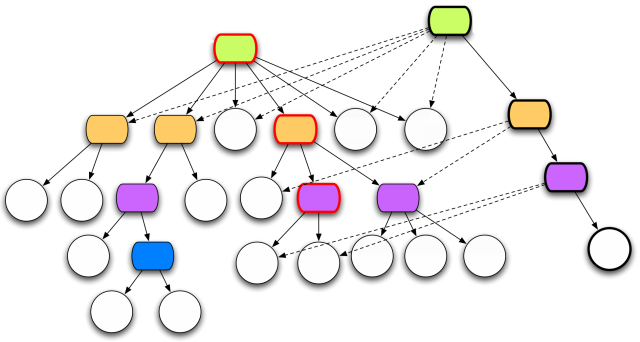
\includegraphics[scale=.65]{images/clojure-trees.png}\\
    \tiny{\textcolor{keyword}{\copyright 2008 Rich Hickey}}
  \end{center}
\end{frame}

\begin{frame}{Collections: Parallel}
  \begin{itemize}[<+->]
    \item \textcolor{hilite}{\tt .par} $\rightarrow$ returns a parallel collection
      \begin{itemize}
        \item $O(1)$ conversion time!
      \end{itemize}
    \item A number of operations can be done concurrently
    \item Uses Fork/Join
    \item Example parallel functions
      \begin{itemize}
        \item {\tt map}
        \item {\tt flatMap}
        \item {\tt foreach}
        \item {\tt filter}
        \item {\tt reduce}
      \end{itemize}
  \end{itemize}
\end{frame}

\begin{frame}{Collections: Demo}
  \begin{center}
    Demo Collections
  \end{center}
\end{frame}

\featureframe{XML}
             {XML Literals!}
             {\featureexample{XML in your code}{xml_literal}}

\featureframe{XML}
             {XML Literals!}
             {\featureexample{XML producing functions}{xml_literal1}}

\featureframe{XML}
             {XML Literals!}
             {\featureexample{XML element splicing}{xml_literal2}}

\featureframe{XML}
             {XML Literals!}
             {\featureexample{Generalized XML splicing}{xml_literal3}}

\featureframe{XML}
             {XML Literals!}
             {\featureexample{Pattern Matching}{xml_literal4}}

\begin{frame}{XML}
  \begin{itemize}[<+->]
    \item XML support generally quite good, but has a fair number of
      warts
    \item EPFL/TypeSafe actively looking to overhaul XML support in
      the language and standard libraries at some point.
      \begin{itemize}
        \item Perhaps with the forthcoming quasi-quoting and macro systems.
      \end{itemize}
    \item Of course there's other library stuff like functions for
      manipulating/querying XML documents.
    \item Of course you can use any other Java or Scala library to
      working with XML (Anti-XML is \emph{very} good
      \tinyurl{http://anti-xml.org/}), but they will not
      \emph{natively} work with the Scala XML types.
  \end{itemize}
\end{frame}

\begin{frame}{Parsing}
  \begin{itemize}[<+->]
    \item Scala library provides a rich \emph{parser combinator
      library}
    \item Can define parsers directly in Scala without using external
      tools like \emph{Antlr} \tinyurl{http://www.antlr.org/}
  \end{itemize}
\end{frame}

\featureframe{Parsing}
             {Parsing Combinators}
             {\featureexample{Simple parser}{parser}}

\begin{frame}{Parsing: Demo}
  \begin{center}
    Demo Parsing Combinators
  \end{center}
\end{frame}

\begin{frame}{Actors}
  \begin{itemize}[<+->]
    \item Actors are a model concurrency based on sending messages
      between logical ``processes''.
    \item Actors are not synonymous with \emph{threads}.  Because of this Actors are lighter-weight than threads and are often managed with a variety of execution strategies.
    \item Scala comes with a respectable Actor library
      \begin{itemize}
        \item Does support local and remote actors
        \item \textcolor{hilite}{Akka} provides a much more robust
          actor implementation.
        \item \textcolor{hilite}{Scalaz} also has a nice (local only)
          actor implementation that is also type-safe.
      \end{itemize}
  \end{itemize}
\end{frame}

\featureframe{Actors}
             {Ping-Pong}
             {\featureexample{Messages}{actor_messages}}

\featureframe{Actors}
             {Ping-Pong}
             {\featureexample{Ponger}{ponger}}

\featureframe{Actors}
             {Ping-Pong}
             {\featureexample{Pinger}{pinger}}

\featureframe{Actors}
             {Ping-Pong}
             {\featureexample{Runner}{runner}}

\begin{frame}{Actors: Demo}
  \begin{center}
    Demo Actors
  \end{center}
\end{frame}

\begin{frame}{Concurrency}
  \begin{itemize}[<+->]
    \item There are a lot of nifty low-level concurrency primitives in the standard Scala library
    \begin{itemize}
      \item Fair to say that many of them will be replaced by higher-performing versions coming from Akka
    \end{itemize}
    \item The most ubiquitous concurrency mechanism in Scala is the \textcolor{hilite}{\emph{Future}}
  \end{itemize}
\end{frame}

\begin{frame}{Concurrency: Futures}
  \begin{itemize}[<+->]
    \item A \textcolor{hilite}{\emph{Future}} represents an asynchronous computation that will eventually yield a value
    \item \textcolor{hilite}{\emph{Futures}} can have a variety of execution strategies
  \end{itemize}
\end{frame}

\featureframe{Futures}
             {Delayed Execution}
             {\featureexample{Bad way}{futures}}

\featureframe{Futures}
             {Monadic composition}
             {\featureexample{Good way}{futures_good}}

\begin{frame}{Futures: Demo}
  \begin{center}
    Demo Futures
  \end{center}
\end{frame}

\begin{frame}{Process Management}
  \begin{itemize}[<+->]
    \item Stole all the goodies from \textcolor{hilite}{SBT}
  \end{itemize}
\end{frame}

\begin{frame}{Process Management: Demo}
  \begin{center}
    Demo Process Management
  \end{center}
\end{frame}

\featureframe{Process Management}
             {Shell interaction}
             {\featureexample{}{process_management}}

\begin{frame}{Swing}
  \begin{itemize}[<+->]
    \item Swing is a desktop UI framework from Java
    \item Provides nice wrappers for this library
  \end{itemize}
\end{frame}

\begin{frame}{Testing}
  \begin{itemize}[<+->]
    \item Bare minimum testing system (much more to come)
    \item Bare minimum benchmarking tool
    \item Several very robust Scala-oriented testing frameworks
    \item Can also use Java testing frameworks
  \end{itemize}
\end{frame}

\featureframe{Testing}
             {Simple test}
             {\featureexample{}{testing}}

\begin{frame}{Testing: Demo}
  \begin{center}
    Demo Testing
  \end{center}
\end{frame}

\end{document}
